\subsection{Overview}

The defining characteristic of the model is the modeling of real rather than synthetic cohorts, all of whom are followed at the individual level. This allows for more heterogeneity in behavior than would be allowed by a cell-based approach. Also, since the HRS interviews both respondent and spouse, we can link records to calculate household-level outcomes such as net income and Social Security retirement benefits, which depend on the outcomes of both spouses. The omission of the population younger than age 51 sacrifices little generality, since the bulk of expenditure on the public programs we consider occurs after age 50. However, we may fail to capture behavioral responses among the young. 

The model has three core components: 
\begin{itemize}
\item The initial cohort module predicts the economic and health outcomes of new cohorts of 51/52 
year-olds. This module takes in data from the Health and Retirement Study (HRS) and trends calculated 
from other sources. It allows us to ``generate'' cohorts as the simulation proceeds, so that we can 
measure outcomes for the age 51+ population in any given year. 
\item The transition module calculates the probabilities of transiting across various health states 
and financial outcomes. The module takes as inputs risk factors such as smoking, weight, age and 
education, along with lagged health and financial states. This allows for a great deal of 
heterogeneity and fairly general feedback effects. The transition probabilities are estimated from 
the longitudinal data in the Health and Retirement Study (HRS). 
\item The policy outcomes module aggregates projections of individual-level outcomes into policy 
outcomes such as taxes, medical care costs, pension benefits paid, and disability benefits. This 
component takes account of public and private program rules to the extent allowed by the available 
outcomes. Because we have access to HRS-linked restricted data from Social Security records and 
employer pension plans, we are able to realistically model retirement benefit receipt. 
\end{itemize}

\begin{figure}[h]
\centering
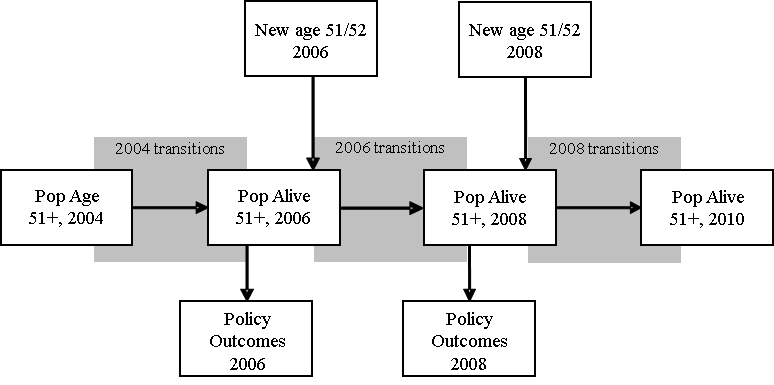
\includegraphics[scale=0.8]{./img/fem_architecture.png}
\caption{Architecture of the FEM}
\label{fig:fem_architecture} 
\end{figure}

Figure \ref{fig:fem_architecture} provides a schematic overview of the model. We start in 2004 with 
an initial population aged 51+ taken from the HRS. We then predict outcomes using our estimated 
transition probabilities (see section \ref{sec:estimation_transition_model}). Those who survive make it to the end of that year, at 
which point we calculate policy outcomes for the year. We then move to the following time period 
(two years later), when a new cohort of 51 and 52 year-olds enters (see section \ref{sec:new_cohorts_model_empirical_strategy}). This entrance 
forms the new age 51+ population, which then proceeds through the transition model as before. This 
process is repeated until we reach the final year of the simulation. 
